\section{量子计算基础}

量子计算理论以量子物理领域的数学物理方法、记号与公式为重要基础;本节将对相关内容进行简单介绍。在学习量子比特与其相关表示的过程中,笔者发现其与本科一年级所学习的线性代数课程有着高度相关性,再一次感受到了理论计算机科学中数学的重要性。

\subsection{量子比特}

量子比特(qubit)是量子计算和量子信息的基本概念。在传统计算机中,经典比特以 0 和 1 两种状态存在。而量子比特也有相对应的两种形态,在 Dirac 表示法中记作 $\ket{0},\ket{1}$,任何一个两态的量子系统都可以实现这一点,例如在氢原子中 $\ket{0},\ket{1}$ 可以代表基态和第一激发态,在质子自旋中可以表示任意方向的 $+\frac{1}{2},-\frac{1}{2}$ 分量。与经典比特不同的是,量子比特除了 $\ket{0}$ 和 $\ket{1}$ 态,还可以处于叠加态(superposition);这是 $\ket{0},\ket{1}$ 两态的一个线性组合,可以记为 \begin{align}\begin{aligned}
        \ket{\psi}=\alpha\ket{0}+\beta\ket{1}\text{\quad 或列向量形式\quad}\ket{\psi}=
        \begin{bmatrix}
            \alpha \\\beta
        \end{bmatrix},
    \end{aligned}\end{align}
其中 $\alpha,\beta\in\mathbb{R}$ (实际上取值域为 $\mathbb{C}^2$,方便起见,这里首先以实数系作为研究对象)且 $|\alpha|^2+|\beta|^2=1$。此时,我们不妨从几何的角度理解这一式子:如果将 $\ket{0}$ 看作 $x$ 方向上的单位向量,$\ket{1}$ 看作 $y$ 方向上的单位向量,那么容易发现,$\ket{\psi}$ 就在单位圆上运动,其模长始终为 $1$。更进一步地,考虑态向量 $\ket{\psi}$ 在这组正交基上的投影,这也就是量子力学中的测量过程: \begin{align*}
    \overrightarrow{\psi_0}=\overrightarrow{0}^T\overrightarrow{\psi}\overrightarrow{0}\Rightarrow\ket{\psi}^{\dagger}\ket{0}\ket{0}=\bra{\psi}\ket{0}\ket{0}=\inner{\psi}{0}\ket{0}=\alpha\ket{0}
\end{align*}
其中,左式是在线性代数中熟知的投影运算形式 $\bm{p}=\bm{u}^{T}\bm{v}\bm{u}$,右式是在量子力学中用 Dirac 记号刻画的更加优美的形式,其中将 $\ket{\psi}^\dagger$ 改写为 $\bra{\psi}$,进而将 $\ket{\psi}\cdot\ket{0}$ 缩写为 $\inner{\psi}{0}$,再考虑投影向量模长的平方 \begin{align*}
    \alpha\bra{0}\cdot\alpha\ket{0}=\alpha^2.
\end{align*}
而在 $\ket{1}$ 上的分量模长平方同理则为 $\beta^2$,这样一来,约束条件 $\alpha^2+\beta^2=1$ 的意义就逐渐清晰:被测量时,其落在 $\ket{0},\ket{1}$ 上的概率之和恰好为 $1$.

在经典比特意义下,$n$ 个比特可以表示 $2^n$ 种不同的状态,在量子比特意义下,也可以通过 $n$ 个量子比特的叠加生成一个 $\dim=2^n$ 的量子比特空间。这个时候需要引入张量积(tensor product)这一概念,这在线性代数课程中尚未涉及,但是可以用一些简单的例子进行理解: \begin{align*}
    \begin{bmatrix}
        1 \\2
    \end{bmatrix}
    \tensor
    \begin{bmatrix}
        3 \\4
    \end{bmatrix}
    =
    \begin{bmatrix}
        1\times \begin{bmatrix}
                    3 \\4
                \end{bmatrix} \\
        2\times \begin{bmatrix}
                    3 \\4
                \end{bmatrix}
    \end{bmatrix}
    =
    \begin{bmatrix}
        3 \\4 \\6 \\8
    \end{bmatrix}.
\end{align*}
于是,叠加两个量子比特可以看作对两个向量进行张量积。这意味着,我们可以首先对基求张量积 \begin{align*}
    \ket{0}\tensor\ket{0}=\ket{00},\ket{0}\tensor\ket{1}=\ket{01},\ket{1}\tensor\ket{0}=\ket{10},\ket{1}\tensor\ket{1}=\ket{11}
\end{align*}
上式可以从许多角度进行理解,例如若置 $\ket{0}=\bm{e}_0=(0,1),\ket{1}=\bm{e}_1=(1,0)$ 为 $\mathbb{R}^2$ 的标准基 ,计算可得 $\ket{00}=(0,0,0,1)=\bm{e}_0,\ket{11}=(1,0,0,0)=\bm{e}_3$ 是 $\mathbb{R}^4$ 的标准基(这里选取 0-base 可以让单位基的角标恰好为 $\ket{}$ 中二进制数的十进制表示)。而后,计算两个任意单量子比特的张量积,例如
\begin{align}\begin{aligned}
        \ket{\psi_1}=\begin{bmatrix}
                         \alpha_1 \\\beta_1
                     \end{bmatrix},
        \ket{\psi_2}=\begin{bmatrix}
                         \alpha_2 \\\beta_2
                     \end{bmatrix}
    \end{aligned}\end{align}
就可以得到
\begin{align}\begin{aligned}
        \ket{\psi_1\psi_2}=\ket{\psi_1}\tensor\ket{\psi_2}=\alpha_1\alpha_2\ket{00}+\alpha_1\beta_2\ket{01}+\alpha_2\beta_1\ket{10}+\beta_1\beta_2\ket{11}=
        \begin{bmatrix}
            \alpha_1\alpha_2 \\\alpha_1\beta_2\\\beta_1\alpha_2\\\beta_1\beta_2
        \end{bmatrix}.
    \end{aligned}\end{align}
特殊地,长度为 $n$ 的全零量子比特表示为 $0^{\tensor n}$,全一量子比特表示为 $1^{\tensor n}$。

\subsection{量子比特门}

每一个量子比特都可以由一个特定维度的单位向量表示,而量子比特之间的运算同样可以用向量变换的手段,即矩阵,进行刻画。值得注意的是,根据 von Neumann 提出的量子力学公设\cite{von2018mathematical},量子比特之间的运算必须是酉变换(unitary transformation),也即,两个沿时间先后顺序出现的量子比特 $\ket{\psi},\ket{\psi'}$ 满足 $\ket{\psi'}=U\,\ket{\psi}$,其中变换矩阵 $U$ 满足其共轭转置与自身的乘积 $U^\dagger U=I$。根据线性代数知识,这蕴含了 $U^\dagger=U=U^{-1}$。在此基础上,我们可以构建出几个常用的合法量子运算门

定义矩阵 $X$ 表示非门 \begin{align}\begin{aligned}
        X=\begin{bmatrix}
              0 & 1 \\
              1 & 0
          \end{bmatrix},\qquad
        \begin{bmatrix}
            \alpha \\\beta
        \end{bmatrix}\mapsto
        \begin{bmatrix}
            \beta \\\alpha
        \end{bmatrix}.
    \end{aligned}\end{align}
显然地,这表示将单量子比特的两位相互交换。这与传统非门是相似的。

定义矩阵 $Z,U$ 表示相位翻转和旋转 \begin{align}
    Z=\begin{bmatrix}
          1 & 0  \\
          0 & -1
      \end{bmatrix}           & ,\qquad
    \begin{bmatrix}
        \alpha \\\beta
    \end{bmatrix}\mapsto
    \begin{bmatrix}
        \alpha \\-\beta
    \end{bmatrix},                      \\
    U=\begin{bmatrix}
          \cos\theta & -\sin\theta \\
          \sin\theta & \cos\theta
      \end{bmatrix} & ,\qquad
    \begin{bmatrix}
        \cos\alpha \\\sin\alpha
    \end{bmatrix}\mapsto
    \begin{bmatrix}
        \cos(\alpha+\theta) \\\sin(\alpha+\theta)
    \end{bmatrix}.
\end{align}

定义矩阵 $H$ 表示 Hadamard 门 \begin{align}\begin{aligned}
        H=\frac{1}{\sqrt{2}}\begin{bmatrix}
                                1 & 1  \\
                                1 & -1
                            \end{bmatrix},\qquad
        \begin{bmatrix}
            \cos\alpha \\
            \sin\alpha
        \end{bmatrix}\mapsto
        \begin{bmatrix}
            \cos(\frac{\pi}{4}-\alpha) \\
            \sin(\frac{\pi}{4}-\alpha)
        \end{bmatrix}
        \label{eq:hadamard}
    \end{aligned}\end{align}
这代表着将一个在 $\mathbb{R}^2$ 的向量沿 $\theta=\frac{\pi}{8}$ 进行对称。于是 \begin{align*}
    H\ket{0}=\frac{\ket{0}+\ket{1}}{\sqrt{2}}=\ket{+}, \\
    H\ket{1}=\frac{\ket{0}-\ket{1}}{\sqrt{2}}=\ket{-}
\end{align*}
这两个向量分别对应了 $\pm\frac{\pi}{4}$,前者位于 $\ket{0},\ket{1}$ 的角平分线上,代表了两者的等概率叠加。因此,Hadamard 门在实际运算中常用于制备叠加态,例如,若需要 $n$ 个量子比特的等概率叠加,即 $\ket{+} $ 的 $n$ 维张量积 \begin{align*}
    \ket{+}^{\tensor n}=\underbrace{\ket{+}\tensor\cdots\tensor\ket{+}}_{\text{$n$ 个 $\ket{+}$}}
\end{align*}
可以考虑对线性算符 $H$ 作张量积并作用于 $\ket{0}$ 上,就得到了 \begin{align*}
    H^{\tensor n}(\ket{0}^{\tensor n})=\ket{+}^{\tensor n}.
\end{align*}

\subsection{量子电路}

在经典计算机中,逻辑电路由一系列逻辑门与电路元件构成,图 \ref{fig:and-or-not-gate} 即为熟知的与或非逻辑门的表示,它们之间相互嵌套组合,构成了经典电子计算机的电路体系。

\begin{figure}[H]
    \centering    %居中
    \subfigure[逻辑与门] %第一张子图
    {
        \label{fig:and-gate}
        \begin{minipage}{4cm}
            \centering          %子图居中
            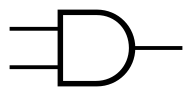
\includegraphics[scale=0.5]{pic/circuit_and.png}   %以pic.jpg的0.5倍大小输出
        \end{minipage}
    }
    \subfigure[逻辑或门] %第一张子图
    {
        \label{fig:or-gate}
        \begin{minipage}{4cm}
            \centering          %子图居中
            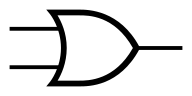
\includegraphics[scale=0.5]{pic/circuit_or.png}   %以pic.jpg的0.5倍大小输出
        \end{minipage}
    }
    \subfigure[逻辑非门] %第一张子图
    {
        \label{fig:not-gate}
        \begin{minipage}{4cm}
            \centering          %子图居中
            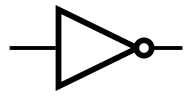
\includegraphics[scale=0.5]{pic/circuit_not.png}   %以pic.jpg的0.5倍大小输出
        \end{minipage}
    }

    \caption{与或非门(ANSI及IEEE标准)} %  %大图名称
    \label{fig:and-or-not-gate}  %图片引用标记
\end{figure}

而在量子电路中的计算则由一系列逻辑门、测量与赋值操作构成。但是,不同于传统电路是用金属线所连接以传递电压信号或电流信号;在量子线路中,线路是由时间所连接,亦即量子比特的状态随着时间自然演化,一直到遇上逻辑门而被操作。另一方面,经典计算机的大多数基本逻辑门(除了非门)都是不可逆的,例如,对于与门,我们不可能从输出信息的每一位恢复到两个输入信息;而量子计算中的每一步操作都是酉变换。刚刚的几个酉变换在量子电路中都有他们的电路元件表示

\begin{figure}[H]
    \centering
    \begin{minipage}{12cm}
        \centering\Qcircuit @C=1em @R=2em @!C @!R {
        \lstick{\hbox to 2em{$\ket{0}$\hss}} & \gate{\hbox{$H$}} & \gate{\hbox{$Z$}} & \gate{\hbox{$X$}} & \gate{\hbox{$U_{-\frac{\pi}{4}}$}} & \meter & \cw \\
        }
    \end{minipage}
\end{figure}
上面的过程中,量子比特的变换过程为 \begin{align*}
    \begin{bmatrix} 0 \\1 \end{bmatrix}\to
    \frac{1}{\sqrt{2}}\begin{bmatrix} 1 \\1 \end{bmatrix}\to
    \frac{1}{\sqrt{2}}\begin{bmatrix} 1 \\-1 \end{bmatrix}\to
    \frac{1}{\sqrt{2}}\begin{bmatrix} -1 \\1 \end{bmatrix}\to
    \begin{bmatrix} 1 \\0 \end{bmatrix}\xrightarrow{\text{measure}}\ket{\psi}
\end{align*}

在实际的计算中,仅仅进行单元操作显然是不够的,因此需要考虑将对单量子比特的操作拓展到多量子比特, 从一种简单的情况出发。现在有两个量子比特,但是仅对其中的一个,即目标量子比特进行操作,另一个作为控制量子比特,决定是否对目标进行否运算, 于是容易得到这一操作的酉矩阵 \begin{align}\begin{aligned}
        U_{\text{CNOT}}=\begin{bmatrix}
                            1 & 0 & 0 & 0 \\
                            0 & 1 & 0 & 0 \\
                            0 & 0 & 0 & 1 \\
                            0 & 0 & 1 & 0
                        \end{bmatrix}
    \end{aligned}\end{align}
当且仅当控制量子比特为 $1$ 时, 目标量子比特通过非门. 可以被表示为 $\ket{A,B}\to\ket{A,B\xor A}$。因此也被形象地表示为
\begin{figure}[H]
    \label{fig:cnot-gate}
    \centering
    \subfigure{
        \begin{minipage}{6cm}
            \centering
            \Qcircuit @C=1em @R=2em @!C @!R {
            &\gate{CNOT} & \qw
            }
        \end{minipage}
    }=
    \subfigure {
        \begin{minipage}{6cm}
            \centering
            \Qcircuit @C=1em @R=2em @!C @!R {
            &\ctrl{1} & \qw\\
            &\targ & \qw
            }
        \end{minipage}
    }
    =
    \subfigure {
        \begin{minipage}{6cm}
            \centering
            \Qcircuit @C=1em @R=2em @!C @!R {
            &\ctrl{1} & \qw\\
            &\gate{X} & \qw
            }
        \end{minipage}
    }
\end{figure}

理论研究证明,任何多量子比特逻辑门可以由受控非门和单量子门组成\cite{nielsen2002quantum},因此,受控非门具有通用性,这也与经典电路中与非门(XAND)的通用性相对应。

\subsection{量子电路的简单应用}

交换两个量子比特的电路可以被表示为

\begin{figure}[H]
    \centering
    \begin{minipage}{12cm}
        \centering
        \Qcircuit @C=1em @R=2em @!C @!R {
        &\ctrl{1}&\targ&\ctrl{1}&\qw\\
        &\targ&\ctrl{-1}&\targ\\
        }
    \end{minipage}
\end{figure}

这是因为容易验证 \begin{align}\begin{aligned}
        \ket{a,b} & \to\ket{a,a\xor b}                              \\
                  & \to\ket{a\xor(a\xor b),a\xor b}=\ket{b,a\xor b} \\
                  & \to\ket{b,(a\xor b)\xor b}=\ket{b,a}.
    \end{aligned}\end{align}

如果在二维 Hadamard 门后面跟着一个 CNOT 门
\begin{figure}[H]
    \centering
    \begin{minipage}{12cm}
        \centering
        \Qcircuit @C=1em @R=2em @!C @!R {
        \lstick{\hbox to 2em{$\ket{00}$\hss}} & \gate{\hbox{$H^{\tensor 2}$}} & \gate{\hbox{$CNOT$}} & \meter & \cw \\
        }
    \end{minipage}
\end{figure}
对四个二维本征态进行计算, 我们会得到 \begin{align}\begin{aligned}
        \ket{0,0}\mapsto\ket{\beta_{0,0}}\frac{\ket{00}+\ket{11}}{\sqrt{2}} \\
        \ket{0,1}\mapsto\ket{\beta_{0,1}}\frac{\ket{01}+\ket{10}}{\sqrt{2}} \\
        \ket{1,0}\mapsto\ket{\beta_{1,0}}\frac{\ket{00}-\ket{11}}{\sqrt{2}} \\
        \ket{1,1}\mapsto\ket{\beta_{1,1}}\frac{\ket{00}-\ket{10}}{\sqrt{2}}
    \end{aligned}\end{align}
概括地 \begin{align}\begin{aligned}
        \ket{\beta_{x,y}}=\frac{\ket{0,y}+(-1)^x\ket{1,\overline{y}}}{\sqrt{2}}.
    \end{aligned}\end{align}

这就是著名的 Bell 态(或 EPR\footnote{Einstein-Podolsky-Rosen} 对),它描述了一种最简单的量子纠缠示例:上面的四个量子比特虽然都具有两个维度,但是在测量中,只要测量了其中的一维,另一维也被唯一地确定了。Bell 态的这一性质使其在超密编码与量子隐形传态的领域扮演着重要的角色。

\subsection{量子电路的设计:Deutsch-Jozsa 算法\label{sec:deutsch}}

Desutsch-Jozsa 算法可由一个简单的游戏进行引入:Alice 从 $0-2^{n}-1$ 中选一个数 $x$ 并将其传送给 Bob。Bob 计算出某个函数 $f(x)$ 的值,可以为 $0$ 或 $1$,并将它传回给 Alice。已知该函数只有可能有两种情况:要么 $f(x)$ 对于所有的 $x$ 均为常数,要么 $f(x)$ 恰好对于一半的 $x$ 取 $0$,一半的取 $1$。Alice 怎样能够最快地判断 $f(x)$ 的类型?

形式化地,已知函数 $f:\{0,1\}^{\otimes n}\rightarrow\{0,1\}$ 一定是下列两种极端形式的一种:
\begin{enumerate}
    \item Constant:$f(x)\equiv 0\text{ or }f(x)\equiv 1$;
    \item Balanced:$f(x)=0~~\text{for half of }\{0,1\}^{\otimes n},\text{ and }f(x)=1~~\text{for the other half}$
\end{enumerate}

问如何用最少的查询次数确定 $f$ 属于二者中的哪一种。

\begin{figure}[H]
    \centering
    \begin{minipage}{12cm}
        \centering
        \def\ingate{\vbox to 3.5em{\hbox to 4em{\tiny$x$\hss $x$}\vss
                    \hbox to 4em{\Large\hss$U_f$\hss}\vss
                    \hbox to 4em{\medmuskip1mu\tiny$x$\hss $y\oplus f(x)$}\vskip-2pt}}
        \Qcircuit @C=1em @R=2em {
        \lstick{\hbox to 2em{$\ket{0}^{\tensor n}$\hss}} & {/}\qw& \qw & \gate{\hbox{$H^{\otimes n}$}} & \multigate{1}{\ingate} & \gate{\hbox{$H^{\otimes n}$}} & \qw & \meter \\
        \lstick{\hbox to 2em{$\ket{0}$\hss}} & \qw & \gate{X} & \gate{H} & \ghost{\ingate} & \qw & \qw & \\
        }
    \end{minipage}
    \caption{Deustch-Jozsa 算法的量子电路}
    \label{fig:deu-joz}
\end{figure}

考虑图 \ref{fig:deu-joz} 所示量子电路,输入 $U_f$ 的初态为 $\ket{+}^{\tensor n}\ket{-}$。考虑初态的前 $n$ 位,设其在某一状态下为 $x$,那么 \begin{align*}
    U_f\ket{x}\ket{-}=\ket{x}\ket{-\tensor f(x)}=(-1)^{f(x)}\ket{x}\ket{-}.
\end{align*}
从而 \begin{align*}
    U_f\ket{+}^{\tensor n}\ket{-}=\sum_{x\in\{0,1\}^{\tensor n}}\frac{(-1)^{f(x)}}{\sqrt{2^n}}\ket{x}\ket{-}.
\end{align*}
另外,容易验证,对于单量子比特门 $H\ket{x}=\sum_{z\in\{0,1\}}(-1)^{xz}\ket{z}/\sqrt{2}$,将这一结果推广到 $n$ 个量子比特上,就有了 \begin{align*}
    H^{\tensor n}\ket{x}=\sum_{z\in\{0,1\}^{\tensor n}}\frac{(-1)^{x\cdot z}}{\sqrt{2^n}}\ket{z}.
\end{align*}
从而 \begin{align*}
    H\left(\sum_{x\in\{0,1\}^{\tensor n}}\frac{(-1)^{f(x)}}{\sqrt{2^n}}\ket{x}\right)=\sum_{x,z\in\{0,1\}^{\tensor n}}\frac{(-1)^{x\cdot z+f(x)}}{2^n}\ket{z}\xrightarrow{\text{measure}}\ket{\psi}
\end{align*}
于是考虑测量结果在 $\bra{0^{\tensor n}}$ 上的分量,即 $z$ 只取 $\ket{0}^{\tensor n}$ 时表达式的值 \begin{align*}
    \inner{0^{\tensor n}}{\psi}=\sum_{x\in\{0,1\}^{\tensor n}}\frac{(-1)^{f(x)}}{2^n}
\end{align*}
因此,当 $f$ 为常值函数时,测量结果必为 $\ket{0}^{\tensor n}$;当 $f$ 为平衡函数时,测量结果不可能出现 $\ket{0}^{\tensor n}$。在整个过程中,运用了 $3$ 个 $n$ 量子比特门,总时间复杂度在 $O(n) = O(\log N)$ 级别,相比于朴素算法 $O(N)$ 的时间开销,量子算法在效率上产生了质的飞跃。Deustch-Jozsa 算法是第一个具有重要意义的量子算法,其出现证明了量子计算在一些方面有着经典计算机无可比拟的性能,为接下来出现的许多量子算法奠基。